\documentclass{article}

\usepackage[utf8]{inputenc}
\usepackage[bottom=2cm, top=2cm, left=2cm, right=2cm]{geometry}
\usepackage{amsmath}
\usepackage{tikz}
\usetikzlibrary{positioning}

\title{Lista 9 - Tabelas Hash
}
\author{Vinícius Couto Tasso}
\date{}

\begin{document}

\maketitle
         
\begin{enumerate}

\item Faça no papel a inserção das chaves 5, 28, 19, 15, 20, 33, 12, 17 e 10 em uma tabela hash com colisões resolvidas por encadeamento. Seja a tabela com 9 posições,  seja a função hash $h(k) = k\ \text{mod}\ M$.

\begin{center}
    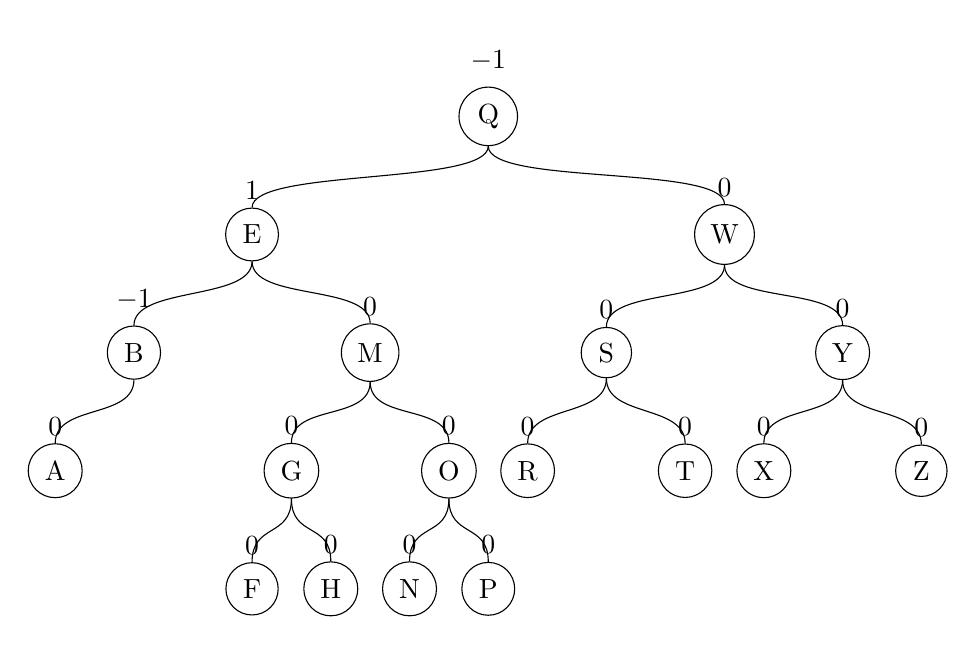
\begin{tikzpicture}[
       edge from parent path=
    {(\tikzparentnode.south) .. controls +(0,-.5) and +(0,.5)
                             .. (\tikzchildnode.north)},
    level 1/.style={sibling distance=6cm},                        
    level 2/.style={sibling distance=3cm},                         
    level 3/.style={sibling distance=2cm},
    level 4/.style={sibling distance=1cm},
   every node/.style={draw,circle},
   label distance=-1mm]
   
\node[label=90:$-1$] {Q}
    child {node[label=90:$1$] {E}
        child {node[label=90:$-1$] {B}
            child {node[label=90:$0$] {A}}
            child[missing]{}
        }
        child {node[label=90:$0$] {M}
            child {node[label=90:$0$] {G}
                child {node[label=90:$0$] {F}}
                child {node[label=90:$0$] {H}}
            }
            child {node[label=90:$0$] {O}
                child {node[label=90:$0$] {N}}
                child {node[label=90:$0$] {P}}
            }
        }
    }   
    child {node[label=90:$0$] {W}
        child {node[label=90:$0$] {S}
            child {node[label=90:$0$] {R}}
            child {node[label=90:$0$] {T}}
            }
        child {node[label=90:$0$] {Y}
            child {node[label=90:$0$] {X}}
            child {node[label=90:$0$] {Z}}
            }
    };

\end{tikzpicture}
\end{center}

\item Faça no papel a inserção das chaves 10, 22, 31, 4, 15, 28, 17, 88, 59 em uma tabela hash de comprimento $m = 11$ usando o endereçamento aberto com a função hash primário $h^\prime(k)=k\ \text{mod}\ m$. Ilustre o resultado destas inserções com a sondagem linear, com a sondagem quadrática com $c_1 = 1$ e $c_2 = 3$, e com a utilização do hash duplo com $h_2(k) = 1 + (k\ \text{mod}\ (m - 1))$. Indique o número total de colisões para cada técnica.

\begin{verbatim}
    Sondagem Linear (7 colisões):
\end{verbatim}

% Insert 10
\begin{center}
    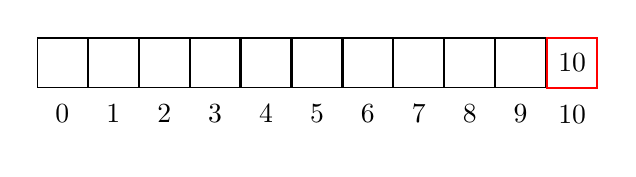
\begin{tikzpicture}
        \tikzstyle{every node}=[draw, minimum size=1.8em]
        
        \matrix[draw=none] {
            \node   (0)    [label=270:$0$] {}; & 
            \node   (1)    [label=270:$1$] {}; &
            \node   (2)    [label=270:$2$] {}; & 
            \node   (3)    [label=270:$3$] {}; &
            \node   (4)    [label=270:$4$] {}; & 
            \node   (5)    [label=270:$5$] {}; &
            \node   (6)    [label=270:$6$] {}; &
            \node   (7)    [label=270:$7$] {}; &
            \node   (8)    [label=270:$8$] {}; &
            \node   (9)    [label=270:$9$] {}; &
            \node   (10)   [label=270:$10$, draw=red, thick] {10}; \\
        };
        
    \end{tikzpicture}
\end{center}

% Insert 22
\begin{center}
    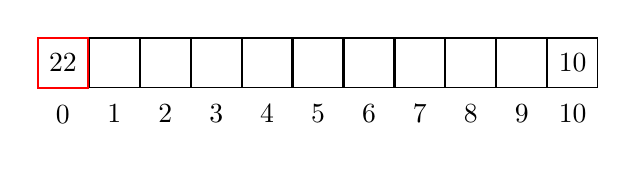
\begin{tikzpicture}
        \tikzstyle{every node}=[draw, minimum size=1.8em]
        
        \matrix[draw=none] {
            \node   (0)    [label=270:$0$, draw=red, thick] {22}; & 
            \node   (1)    [label=270:$1$] {}; &
            \node   (2)    [label=270:$2$] {}; & 
            \node   (3)    [label=270:$3$] {}; &
            \node   (4)    [label=270:$4$] {}; & 
            \node   (5)    [label=270:$5$] {}; &
            \node   (6)    [label=270:$6$] {}; &
            \node   (7)    [label=270:$7$] {}; &
            \node   (8)    [label=270:$8$] {}; &
            \node   (9)    [label=270:$9$] {}; &
            \node   (10)   [label=270:$10$] {10}; \\
        };
        
    \end{tikzpicture}
\end{center}

% Insert 31
\begin{center}
    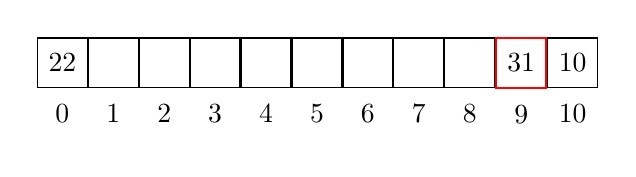
\begin{tikzpicture}
        \tikzstyle{every node}=[draw, minimum size=1.8em]
        
        \matrix[draw=none] {
            \node   (0)    [label=270:$0$] {22}; & 
            \node   (1)    [label=270:$1$] {}; &
            \node   (2)    [label=270:$2$] {}; & 
            \node   (3)    [label=270:$3$] {}; &
            \node   (4)    [label=270:$4$] {}; & 
            \node   (5)    [label=270:$5$] {}; &
            \node   (6)    [label=270:$6$] {}; &
            \node   (7)    [label=270:$7$] {}; &
            \node   (8)    [label=270:$8$] {}; &
            \node   (9)    [label=270:$9$, draw=red, thick] {31}; &
            \node   (10)   [label=270:$10$] {10}; \\
        };
        
    \end{tikzpicture}
\end{center}

% Insert 4
\begin{center}
    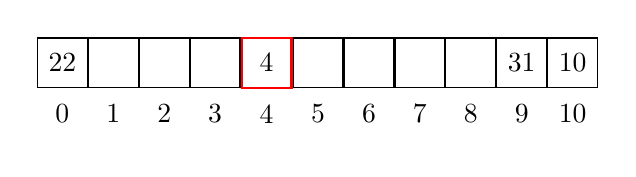
\begin{tikzpicture}
        \tikzstyle{every node}=[draw, minimum size=1.8em]
        
        \matrix[draw=none] {
            \node   (0)    [label=270:$0$] {22}; & 
            \node   (1)    [label=270:$1$] {}; &
            \node   (2)    [label=270:$2$] {}; & 
            \node   (3)    [label=270:$3$] {}; &
            \node   (4)    [label=270:$4$, draw=red, thick] {4}; & 
            \node   (5)    [label=270:$5$] {}; &
            \node   (6)    [label=270:$6$] {}; &
            \node   (7)    [label=270:$7$] {}; &
            \node   (8)    [label=270:$8$] {}; &
            \node   (9)    [label=270:$9$] {31}; &
            \node   (10)   [label=270:$10$] {10}; \\
        };
        
    \end{tikzpicture}
\end{center}

% Insert 15
\begin{center}
    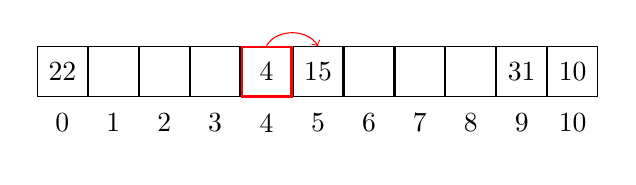
\begin{tikzpicture}
        \tikzstyle{every node}=[draw, minimum size=1.8em]
        
        \matrix[draw=none] {
            \node   (0)    [label=270:$0$] {22}; & 
            \node   (1)    [label=270:$1$] {}; &
            \node   (2)    [label=270:$2$] {}; & 
            \node   (3)    [label=270:$3$] {}; &
            \node   (4)    [label=270:$4$, draw=red, thick] {4}; & 
            \node   (5)    [label=270:$5$] {15}; &
            \node   (6)    [label=270:$6$] {}; &
            \node   (7)    [label=270:$7$] {}; &
            \node   (8)    [label=270:$8$] {}; &
            \node   (9)    [label=270:$9$] {31}; &
            \node   (10)   [label=270:$10$] {10}; \\
        };
        
        \draw[->, red, out=60, in=120] (4.north) to (5.north);
        
    \end{tikzpicture}
\end{center}

% Insert 28
\begin{center}
    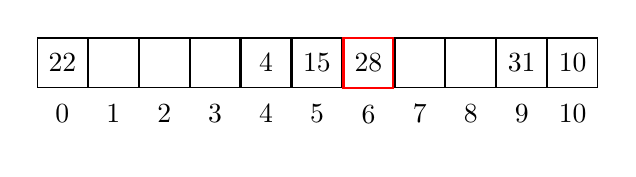
\begin{tikzpicture}
        \tikzstyle{every node}=[draw, minimum size=1.8em]
        
        \matrix[draw=none] {
            \node   (0)    [label=270:$0$] {22}; & 
            \node   (1)    [label=270:$1$] {}; &
            \node   (2)    [label=270:$2$] {}; & 
            \node   (3)    [label=270:$3$] {}; &
            \node   (4)    [label=270:$4$] {4}; & 
            \node   (5)    [label=270:$5$] {15}; &
            \node   (6)    [label=270:$6$, draw=red, thick] {28}; &
            \node   (7)    [label=270:$7$] {}; &
            \node   (8)    [label=270:$8$] {}; &
            \node   (9)    [label=270:$9$] {31}; &
            \node   (10)   [label=270:$10$] {10}; \\
        };
        
    \end{tikzpicture}
\end{center}

% Insert 17
\begin{center}
    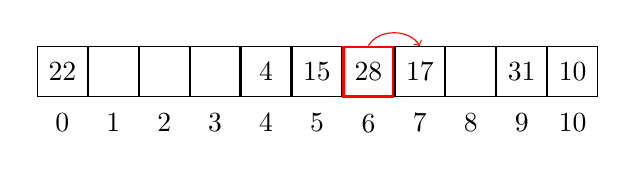
\begin{tikzpicture}
        \tikzstyle{every node}=[draw, minimum size=1.8em]
        
        \matrix[draw=none] {
            \node   (0)    [label=270:$0$] {22}; & 
            \node   (1)    [label=270:$1$] {}; &
            \node   (2)    [label=270:$2$] {}; & 
            \node   (3)    [label=270:$3$] {}; &
            \node   (4)    [label=270:$4$] {4}; & 
            \node   (5)    [label=270:$5$] {15}; &
            \node   (6)    [label=270:$6$, draw=red, thick] {28}; &
            \node   (7)    [label=270:$7$] {17}; &
            \node   (8)    [label=270:$8$] {}; &
            \node   (9)    [label=270:$9$] {31}; &
            \node   (10)   [label=270:$10$] {10}; \\
        };
        
        \draw[->, red, out=60, in=120] (6.north) to (7.north);
        
    \end{tikzpicture}
\end{center}

% Insert 88
\begin{center}
    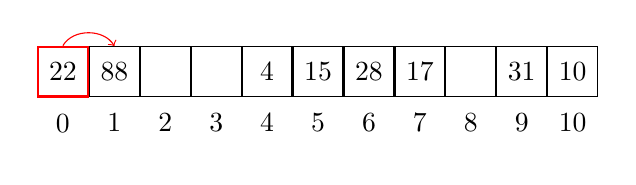
\begin{tikzpicture}
        \tikzstyle{every node}=[draw, minimum size=1.8em]
        
        \matrix[draw=none] {
            \node   (0)    [label=270:$0$, draw=red, thick] {22}; & 
            \node   (1)    [label=270:$1$] {88}; &
            \node   (2)    [label=270:$2$] {}; & 
            \node   (3)    [label=270:$3$] {}; &
            \node   (4)    [label=270:$4$] {4}; & 
            \node   (5)    [label=270:$5$] {15}; &
            \node   (6)    [label=270:$6$] {28}; &
            \node   (7)    [label=270:$7$] {17}; &
            \node   (8)    [label=270:$8$] {}; &
            \node   (9)    [label=270:$9$] {31}; &
            \node   (10)   [label=270:$10$] {10}; \\
        };
        
        \draw[->, red, out=60, in=120] (0.north) to (1.north);
        
    \end{tikzpicture}
\end{center}

% Insert 59
\begin{center}
    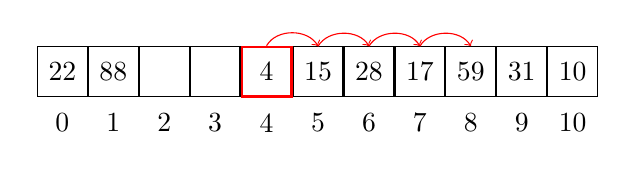
\begin{tikzpicture}
        \tikzstyle{every node}=[draw, minimum size=1.8em]
        
        \matrix[draw=none] {
            \node   (0)    [label=270:$0$] {22}; & 
            \node   (1)    [label=270:$1$] {88}; &
            \node   (2)    [label=270:$2$] {}; & 
            \node   (3)    [label=270:$3$] {}; &
            \node   (4)    [label=270:$4$, draw=red, thick] {4}; & 
            \node   (5)    [label=270:$5$] {15}; &
            \node   (6)    [label=270:$6$] {28}; &
            \node   (7)    [label=270:$7$] {17}; &
            \node   (8)    [label=270:$8$] {59}; &
            \node   (9)    [label=270:$9$] {31}; &
            \node   (10)   [label=270:$10$] {10}; \\
        };
    
        \path[->, red]  (4.north) edge [out=60, in=120] (5.north)
                        (5.north) edge [out=60, in=120] (6.north)
                        (6.north) edge [out=60, in=120] (7.north)
                        (7.north) edge [out=60, in=120] (8.north);
        
    \end{tikzpicture}
\end{center}

\begin{verbatim}
    Sondagem Quadrática (14 colisões):
\end{verbatim}

% Insert 10
\begin{center}
    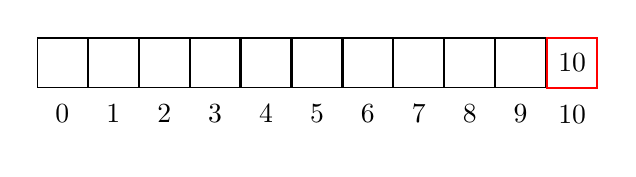
\begin{tikzpicture}
        \tikzstyle{every node}=[draw, minimum size=1.8em]
        
        \matrix[draw=none] {
            \node   (0)    [label=270:$0$] {}; & 
            \node   (1)    [label=270:$1$] {}; &
            \node   (2)    [label=270:$2$] {}; & 
            \node   (3)    [label=270:$3$] {}; &
            \node   (4)    [label=270:$4$] {}; & 
            \node   (5)    [label=270:$5$] {}; &
            \node   (6)    [label=270:$6$] {}; &
            \node   (7)    [label=270:$7$] {}; &
            \node   (8)    [label=270:$8$] {}; &
            \node   (9)    [label=270:$9$] {}; &
            \node   (10)   [label=270:$10$, draw=red, thick] {10}; \\
        };
        
    \end{tikzpicture}
\end{center}

% Insert 22
\begin{center}
    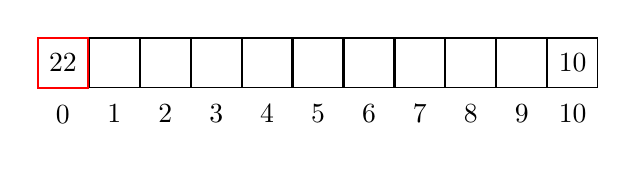
\begin{tikzpicture}
        \tikzstyle{every node}=[draw, minimum size=1.8em]
        
        \matrix[draw=none] {
            \node   (0)    [label=270:$0$, draw=red, thick] {22}; & 
            \node   (1)    [label=270:$1$] {}; &
            \node   (2)    [label=270:$2$] {}; & 
            \node   (3)    [label=270:$3$] {}; &
            \node   (4)    [label=270:$4$] {}; & 
            \node   (5)    [label=270:$5$] {}; &
            \node   (6)    [label=270:$6$] {}; &
            \node   (7)    [label=270:$7$] {}; &
            \node   (8)    [label=270:$8$] {}; &
            \node   (9)    [label=270:$9$] {}; &
            \node   (10)   [label=270:$10$] {10}; \\
        };
        
    \end{tikzpicture}
\end{center}

% Insert 31
\begin{center}
    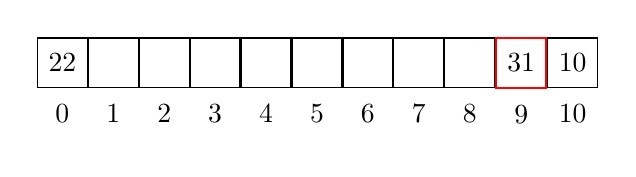
\begin{tikzpicture}
        \tikzstyle{every node}=[draw, minimum size=1.8em]
        
        \matrix[draw=none] {
            \node   (0)    [label=270:$0$] {22}; & 
            \node   (1)    [label=270:$1$] {}; &
            \node   (2)    [label=270:$2$] {}; & 
            \node   (3)    [label=270:$3$] {}; &
            \node   (4)    [label=270:$4$] {}; & 
            \node   (5)    [label=270:$5$] {}; &
            \node   (6)    [label=270:$6$] {}; &
            \node   (7)    [label=270:$7$] {}; &
            \node   (8)    [label=270:$8$] {}; &
            \node   (9)    [label=270:$9$, draw=red, thick] {31}; &
            \node   (10)   [label=270:$10$] {10}; \\
        };
        
    \end{tikzpicture}
\end{center}

% Insert 4
\begin{center}
    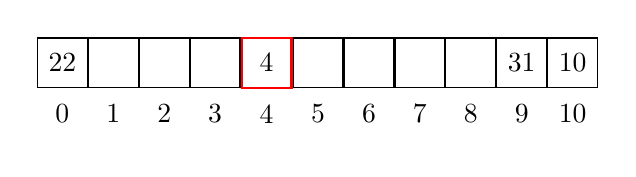
\begin{tikzpicture}
        \tikzstyle{every node}=[draw, minimum size=1.8em]
        
        \matrix[draw=none] {
            \node   (0)    [label=270:$0$] {22}; & 
            \node   (1)    [label=270:$1$] {}; &
            \node   (2)    [label=270:$2$] {}; & 
            \node   (3)    [label=270:$3$] {}; &
            \node   (4)    [label=270:$4$, draw=red, thick] {4}; & 
            \node   (5)    [label=270:$5$] {}; &
            \node   (6)    [label=270:$6$] {}; &
            \node   (7)    [label=270:$7$] {}; &
            \node   (8)    [label=270:$8$] {}; &
            \node   (9)    [label=270:$9$] {31}; &
            \node   (10)   [label=270:$10$] {10}; \\
        };
        
    \end{tikzpicture}
\end{center}

% Insert 15
\begin{center}
    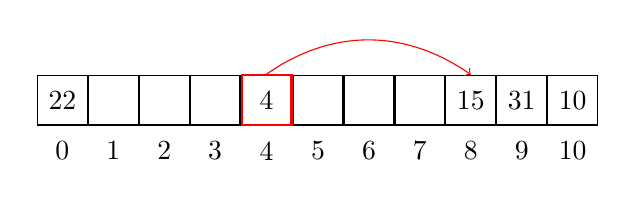
\begin{tikzpicture}
        \tikzstyle{every node}=[draw, minimum size=1.8em]
        
        \matrix[draw=none] {
            \node   (0)    [label=270:$0$] {22}; & 
            \node   (1)    [label=270:$1$] {}; &
            \node   (2)    [label=270:$2$] {}; & 
            \node   (3)    [label=270:$3$] {}; &
            \node   (4)    [label=270:$4$, draw=red, thick] {4}; & 
            \node   (5)    [label=270:$5$] {}; &
            \node   (6)    [label=270:$6$] {}; &
            \node   (7)    [label=270:$7$] {}; &
            \node   (8)    [label=270:$8$] {15}; &
            \node   (9)    [label=270:$9$] {31}; &
            \node   (10)   [label=270:$10$] {10}; \\
        };
        
        \draw[->, red, out=35, in=145] (4.north) to (8.north);
        
    \end{tikzpicture}
\end{center}

% Insert 28
\begin{center}
    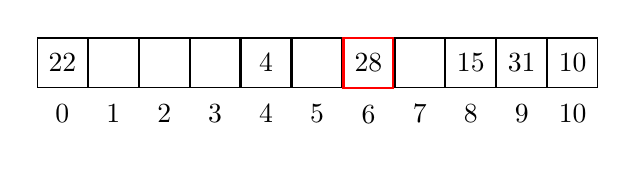
\begin{tikzpicture}
        \tikzstyle{every node}=[draw, minimum size=1.8em]
        
        \matrix[draw=none] {
            \node   (0)    [label=270:$0$] {22}; & 
            \node   (1)    [label=270:$1$] {}; &
            \node   (2)    [label=270:$2$] {}; & 
            \node   (3)    [label=270:$3$] {}; &
            \node   (4)    [label=270:$4$] {4}; & 
            \node   (5)    [label=270:$5$] {}; &
            \node   (6)    [label=270:$6$, draw=red, thick] {28}; &
            \node   (7)    [label=270:$7$] {}; &
            \node   (8)    [label=270:$8$] {15}; &
            \node   (9)    [label=270:$9$] {31}; &
            \node   (10)   [label=270:$10$] {10}; \\
        };
        
    \end{tikzpicture}
\end{center}

% Insert 17
\begin{center}
    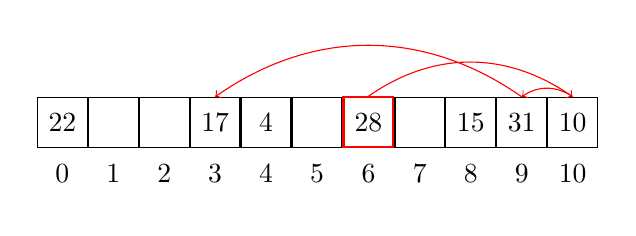
\begin{tikzpicture}
        \tikzstyle{every node}=[draw, minimum size=1.8em]
        
        \matrix[draw=none] {
            \node   (0)    [label=270:$0$] {22}; & 
            \node   (1)    [label=270:$1$] {}; &
            \node   (2)    [label=270:$2$] {}; & 
            \node   (3)    [label=270:$3$] {17}; &
            \node   (4)    [label=270:$4$] {4}; & 
            \node   (5)    [label=270:$5$] {}; &
            \node   (6)    [label=270:$6$, draw=red, thick] {28}; &
            \node   (7)    [label=270:$7$] {}; &
            \node   (8)    [label=270:$8$] {15}; &
            \node   (9)    [label=270:$9$] {31}; &
            \node   (10)   [label=270:$10$] {10}; \\
        };
        
        \path[->, red]  (6.north) edge [out=35, in=145] (10.north)
                        (10.north) edge [out=145, in=35] (9.north)
                        (9.north) edge [out=145, in=35] (3.north);
        
    \end{tikzpicture}
\end{center}

% Insert 88
\begin{center}
    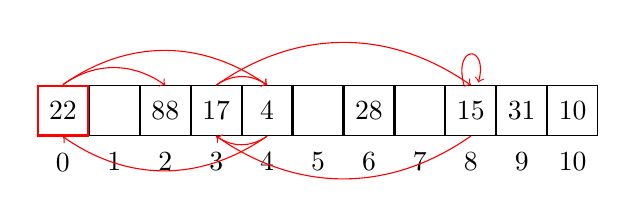
\begin{tikzpicture}
        \tikzstyle{every node}=[draw, minimum size=1.8em]
        
        \matrix[draw=none] {
            \node   (0)    [label=270:$0$, draw=red, thick] {22}; & 
            \node   (1)    [label=270:$1$] {}; &
            \node   (2)    [label=270:$2$] {88}; & 
            \node   (3)    [label=270:$3$] {17}; &
            \node   (4)    [label=270:$4$] {4}; & 
            \node   (5)    [label=270:$5$] {}; &
            \node   (6)    [label=270:$6$] {28}; &
            \node   (7)    [label=270:$7$] {}; &
            \node   (8)    [label=270:$8$] {15}; &
            \node   (9)    [label=270:$9$] {31}; &
            \node   (10)   [label=270:$10$] {10}; \\
        };
        
        \path[->, red]  (0.north) edge [out=35, in=145] (4.north)
                        (4.south) edge [out=-145, in=-35] (3.south)
                        (3.north) edge [out=35, in=145] (8.north)
                        (8) edge [loop above] ()
                        (8.south) edge [out=-145, in=-35] (3.south)
                        (3.north) edge [out=35, in=145] (4.north)
                        (4.south) edge [out=-145, in=-35] (0.south)
                        (0.north) edge [out=35, in=145] (2.north);
        
    \end{tikzpicture}
\end{center}

% Insert 59
\begin{center}
    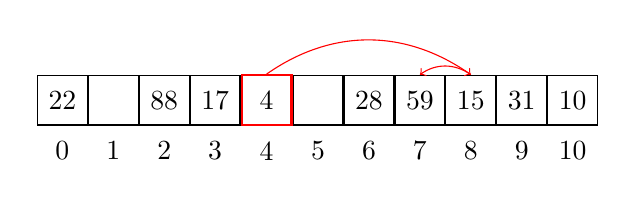
\begin{tikzpicture}
        \tikzstyle{every node}=[draw, minimum size=1.8em]
        
        \matrix[draw=none] {
            \node   (0)    [label=270:$0$] {22}; & 
            \node   (1)    [label=270:$1$] {}; &
            \node   (2)    [label=270:$2$] {88}; & 
            \node   (3)    [label=270:$3$] {17}; &
            \node   (4)    [label=270:$4$, draw=red, thick] {4}; & 
            \node   (5)    [label=270:$5$] {}; &
            \node   (6)    [label=270:$6$] {28}; &
            \node   (7)    [label=270:$7$] {59}; &
            \node   (8)    [label=270:$8$] {15}; &
            \node   (9)    [label=270:$9$] {31}; &
            \node   (10)   [label=270:$10$] {10}; \\
        };
        
        \path[->, red]  (4.north) edge [out=35, in=145] (8.north)
                        (8.north) edge [out=145, in=35] (7.north);
        
    \end{tikzpicture}
\end{center}

\begin{verbatim}
    Hash duplo (7 colisões):
\end{verbatim}

% Insert 10
\begin{center}
    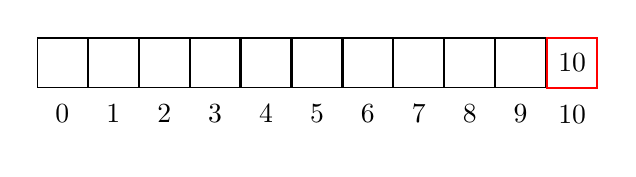
\begin{tikzpicture}
        \tikzstyle{every node}=[draw, minimum size=1.8em]
        
        \matrix[draw=none] {
            \node   (0)    [label=270:$0$] {}; & 
            \node   (1)    [label=270:$1$] {}; &
            \node   (2)    [label=270:$2$] {}; & 
            \node   (3)    [label=270:$3$] {}; &
            \node   (4)    [label=270:$4$] {}; & 
            \node   (5)    [label=270:$5$] {}; &
            \node   (6)    [label=270:$6$] {}; &
            \node   (7)    [label=270:$7$] {}; &
            \node   (8)    [label=270:$8$] {}; &
            \node   (9)    [label=270:$9$] {}; &
            \node   (10)   [label=270:$10$, draw=red, thick] {10}; \\
        };
        
    \end{tikzpicture}
\end{center}

% Insert 22
\begin{center}
    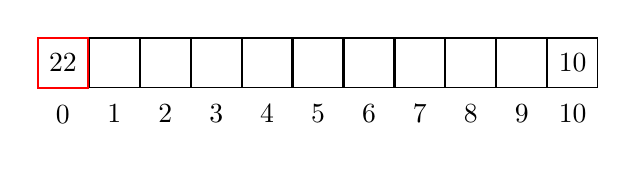
\begin{tikzpicture}
        \tikzstyle{every node}=[draw, minimum size=1.8em]
        
        \matrix[draw=none] {
            \node   (0)    [label=270:$0$, draw=red, thick] {22}; & 
            \node   (1)    [label=270:$1$] {}; &
            \node   (2)    [label=270:$2$] {}; & 
            \node   (3)    [label=270:$3$] {}; &
            \node   (4)    [label=270:$4$] {}; & 
            \node   (5)    [label=270:$5$] {}; &
            \node   (6)    [label=270:$6$] {}; &
            \node   (7)    [label=270:$7$] {}; &
            \node   (8)    [label=270:$8$] {}; &
            \node   (9)    [label=270:$9$] {}; &
            \node   (10)   [label=270:$10$] {10}; \\
        };
        
    \end{tikzpicture}
\end{center}

% Insert 31
\begin{center}
    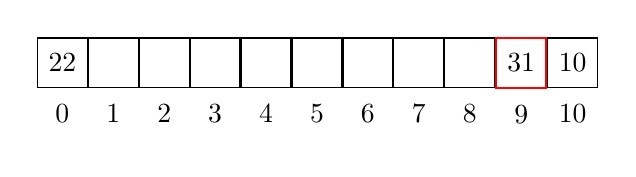
\begin{tikzpicture}
        \tikzstyle{every node}=[draw, minimum size=1.8em]
        
        \matrix[draw=none] {
            \node   (0)    [label=270:$0$] {22}; & 
            \node   (1)    [label=270:$1$] {}; &
            \node   (2)    [label=270:$2$] {}; & 
            \node   (3)    [label=270:$3$] {}; &
            \node   (4)    [label=270:$4$] {}; & 
            \node   (5)    [label=270:$5$] {}; &
            \node   (6)    [label=270:$6$] {}; &
            \node   (7)    [label=270:$7$] {}; &
            \node   (8)    [label=270:$8$] {}; &
            \node   (9)    [label=270:$9$, draw=red, thick] {31}; &
            \node   (10)   [label=270:$10$] {10}; \\
        };
        
    \end{tikzpicture}
\end{center}

% Insert 4
\begin{center}
    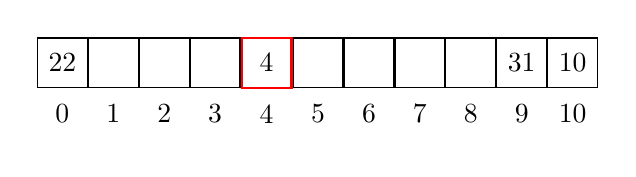
\begin{tikzpicture}
        \tikzstyle{every node}=[draw, minimum size=1.8em]
        
        \matrix[draw=none] {
            \node   (0)    [label=270:$0$] {22}; & 
            \node   (1)    [label=270:$1$] {}; &
            \node   (2)    [label=270:$2$] {}; & 
            \node   (3)    [label=270:$3$] {}; &
            \node   (4)    [label=270:$4$, draw=red, thick] {4}; & 
            \node   (5)    [label=270:$5$] {}; &
            \node   (6)    [label=270:$6$] {}; &
            \node   (7)    [label=270:$7$] {}; &
            \node   (8)    [label=270:$8$] {}; &
            \node   (9)    [label=270:$9$] {31}; &
            \node   (10)   [label=270:$10$] {10}; \\
        };
        
    \end{tikzpicture}
\end{center}

% Insert 15
\begin{center}
    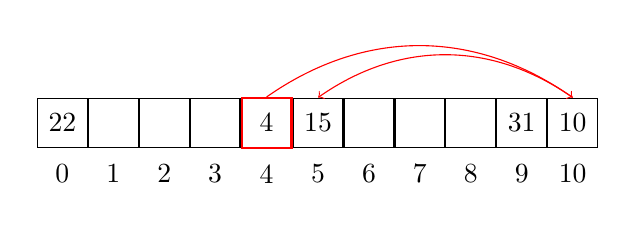
\begin{tikzpicture}
        \tikzstyle{every node}=[draw, minimum size=1.8em]
        
        \matrix[draw=none] {
            \node   (0)    [label=270:$0$] {22}; & 
            \node   (1)    [label=270:$1$] {}; &
            \node   (2)    [label=270:$2$] {}; & 
            \node   (3)    [label=270:$3$] {}; &
            \node   (4)    [label=270:$4$, draw=red, thick] {4}; & 
            \node   (5)    [label=270:$5$] {15}; &
            \node   (6)    [label=270:$6$] {}; &
            \node   (7)    [label=270:$7$] {}; &
            \node   (8)    [label=270:$8$] {}; &
            \node   (9)    [label=270:$9$] {31}; &
            \node   (10)   [label=270:$10$] {10}; \\
        };
        
        \path[->, red]  (4.north) edge [out=35, in=145] (10.north)
                        (10.north) edge [out=145, in=35] (5.north);
        
    \end{tikzpicture}
\end{center}

% Insert 28
\begin{center}
    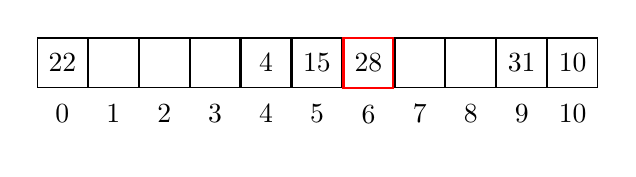
\begin{tikzpicture}
        \tikzstyle{every node}=[draw, minimum size=1.8em]
        
        \matrix[draw=none] {
            \node   (0)    [label=270:$0$] {22}; & 
            \node   (1)    [label=270:$1$] {}; &
            \node   (2)    [label=270:$2$] {}; & 
            \node   (3)    [label=270:$3$] {}; &
            \node   (4)    [label=270:$4$] {4}; & 
            \node   (5)    [label=270:$5$] {15}; &
            \node   (6)    [label=270:$6$, draw=red, thick] {28}; &
            \node   (7)    [label=270:$7$] {}; &
            \node   (8)    [label=270:$8$] {}; &
            \node   (9)    [label=270:$9$] {31}; &
            \node   (10)   [label=270:$10$] {10}; \\
        };
        
    \end{tikzpicture}
\end{center}

% Insert 17
\begin{center}
    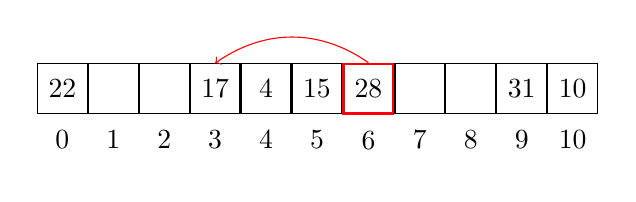
\begin{tikzpicture}
        \tikzstyle{every node}=[draw, minimum size=1.8em]
        
        \matrix[draw=none] {
            \node   (0)    [label=270:$0$] {22}; & 
            \node   (1)    [label=270:$1$] {}; &
            \node   (2)    [label=270:$2$] {}; & 
            \node   (3)    [label=270:$3$] {17}; &
            \node   (4)    [label=270:$4$] {4}; & 
            \node   (5)    [label=270:$5$] {15}; &
            \node   (6)    [label=270:$6$, draw=red, thick] {28}; &
            \node   (7)    [label=270:$7$] {}; &
            \node   (8)    [label=270:$8$] {}; &
            \node   (9)    [label=270:$9$] {31}; &
            \node   (10)   [label=270:$10$] {10}; \\
        };
        
        \path[->, red] (6.north) edge [out=145, in=35] (3.north);
        
    \end{tikzpicture}
\end{center}

% Insert 88
\begin{center}
    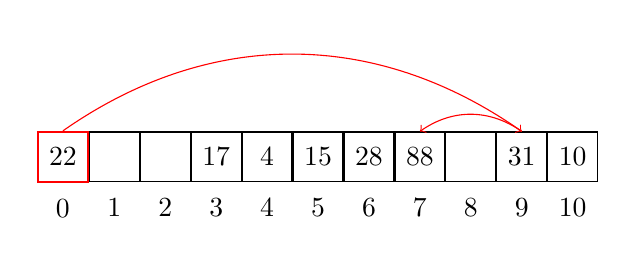
\begin{tikzpicture}
        \tikzstyle{every node}=[draw, minimum size=1.8em]
        
        \matrix[draw=none] {
            \node   (0)    [label=270:$0$, draw=red, thick] {22}; & 
            \node   (1)    [label=270:$1$] {}; &
            \node   (2)    [label=270:$2$] {}; & 
            \node   (3)    [label=270:$3$] {17}; &
            \node   (4)    [label=270:$4$] {4}; & 
            \node   (5)    [label=270:$5$] {15}; &
            \node   (6)    [label=270:$6$] {28}; &
            \node   (7)    [label=270:$7$] {88}; &
            \node   (8)    [label=270:$8$] {}; &
            \node   (9)    [label=270:$9$] {31}; &
            \node   (10)   [label=270:$10$] {10}; \\
        };
        
        \path[->, red] (0.north) edge [out=35, in=145] (9.north)
                       (9.north) edge [out=145, in=35] (7.north);
        
    \end{tikzpicture}
\end{center}

% Insert 59
\begin{center}
    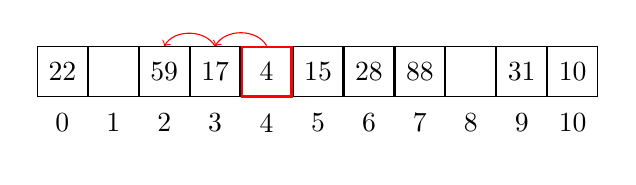
\begin{tikzpicture}
        \tikzstyle{every node}=[draw, minimum size=1.8em]
        
        \matrix[draw=none] {
            \node   (0)    [label=270:$0$] {22}; & 
            \node   (1)    [label=270:$1$] {}; &
            \node   (2)    [label=270:$2$] {59}; & 
            \node   (3)    [label=270:$3$] {17}; &
            \node   (4)    [label=270:$4$, draw=red, thick] {4}; & 
            \node   (5)    [label=270:$5$] {15}; &
            \node   (6)    [label=270:$6$] {28}; &
            \node   (7)    [label=270:$7$] {88}; &
            \node   (8)    [label=270:$8$] {}; &
            \node   (9)    [label=270:$9$] {31}; &
            \node   (10)   [label=270:$10$] {10}; \\
        };
        
        \path[->, red] (4.north) edge [out=120, in=60] (3.north)
                       (3.north) edge [out=120, in=60] (2.north);
        
        
    \end{tikzpicture}
\end{center}

\end{enumerate}

\end{document}
